% Preamble
% ---
\documentclass[a4paper]{article}

% Packages
% ---
\usepackage{bm}
\usepackage[spanish,es-nodecimaldot]{babel}
\usepackage[utf8]{inputenc}
\usepackage[T1]{fontenc}
\usepackage{parskip}
\usepackage{fancyhdr}
\usepackage{mathtools}
\usepackage{amsmath}
\usepackage[htt]{hyphenat}
\usepackage{capt-of}
\usepackage{lscape}
\usepackage{graphicx}
\graphicspath{ {./images/} }

% Pagestyles
% ---
\pagestyle{fancy}
\rhead{Roselló Beneitez, N. U.; Roselló Oviedo, M.}
\lhead{APR: Mixtura de gaussianas}
\fancyfoot[C]{\thepage}

% Main
% ---
\begin{document}

\author{Roselló Beneitez, N. U.; Roselló Oviedo, M.}
\title{APR: Práctica sobre Mixtura de gaussianas}
\date{6 de Enero de 2020}
\maketitle{}
\thispagestyle{empty}

\newpage
\tableofcontents
\listoffigures

\newpage
\section{Descripción de la práctica}
\quad En esta práctica se ha realizado una clasificación para la base de datos de dígitos \textit{MNIST} mediante diversas técnicas: un clasificador multinomial, un clasificador gaussiano y un clasificador basado en mixtura de gaussianas.

\quad Tanto el clasificador multinomial como el clasificador gaussiano se nos proporcionaban ya implementados, por lo que solo ha bastado ejecutar estos programas para obtener los resultados (véase “Resultados obtenidos”).

\quad En el modelo de clasificador basado en mixtura de gaussianas, se ha empleado el algoritmo \textit{EM} (Esperanza - Maximización) para el aprendizaje de las muestras por cada componente. Para ello se ha tenido que implementar únicamente el paso \textit{M}, puesto que el paso E ya se daba completo.

\section{Un pequeño ejercicio completo de aprendizaje}

\subsection{Ejercicio 4.1}
\quad Cuando el valor del suavizado ($ \alpha $) se mantiene constante e igual a 1, los resultados son los siguientes:
$ \\ $
\begin{figure}[!h]
	  \centering
	  \begin{minipage}[b]{0.25\textwidth}
	   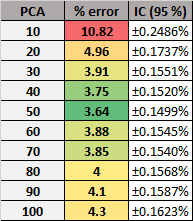
\includegraphics[width=100px]{1_41_1}
	  \end{minipage}
	  \hfill
	  \begin{minipage}[b]{0.65\textwidth}
	    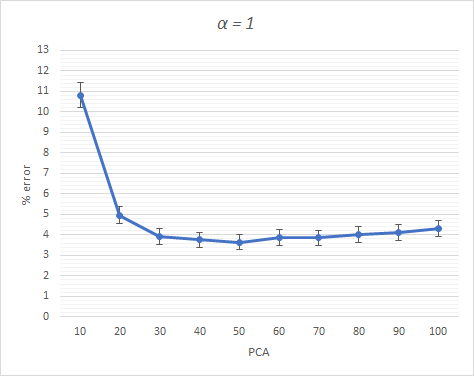
\includegraphics[width=250px]{1_41_2}
	  \end{minipage}
\end{figure}
\begin{center}
\captionof{figure}{Error e IC 95\% en función de PCA para $\alpha = 1$}
\end{center}

\subsection{Ejercicio 4.2}
\quad Se ha experimentado con valores del suavizado en el conjunto {0.001, 0.01, 0.1, 0.2, 0.5, 0.9, 0.95, 0.99}. Los resultados se muestran a continuación:
\begin{center}
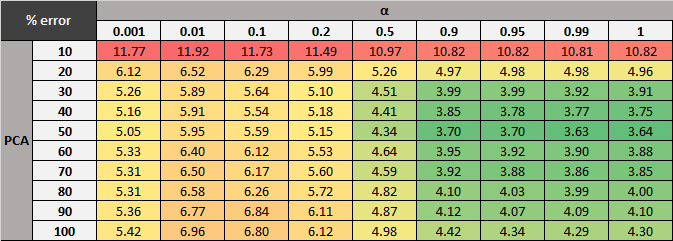
\includegraphics[width=\textwidth]{1_42_1}

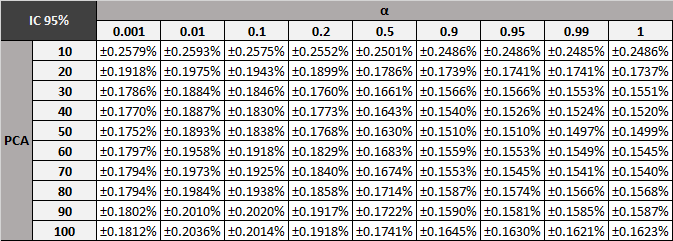
\includegraphics[width=\textwidth]{1_42_2}

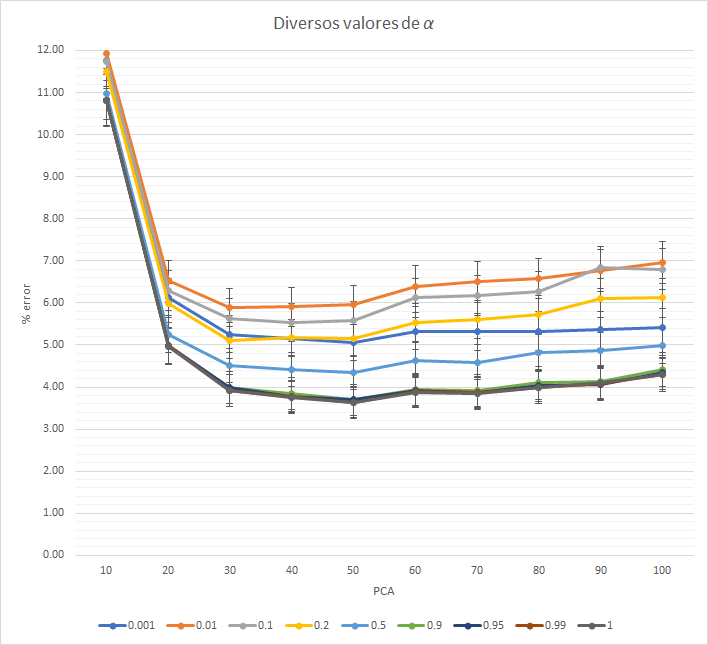
\includegraphics[width=\textwidth]{1_42_3}
\captionof{figure}{Error e IC 95\% en función de PCA para diversos valores de $\alpha$}
\end{center}

\section{Aplicación de SVM a MNIST}

\subsection{Ejericio 5.1}
\quad El código adjunto muestra el paso M. Las ecuaciones están debidamente comentadas como el número de ecuación que implementan.

\subsection{Ejericio 5.2}
\quad Puesto que se ha observado que aplicar un suavizado menor a 0.5 carece de sentido, y con el fin de ahorrar ejecuciones, los valores de $\alpha$ han cambiado: ahora están en el conjunto $\lbrace 0.5, 0.7, 0.9, 0.95, 0.99 \rbrace$.
$ \\ $
\begin{center}
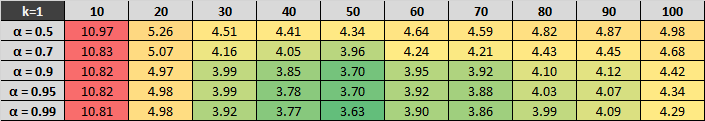
\includegraphics[width=\textwidth]{1_52_1}

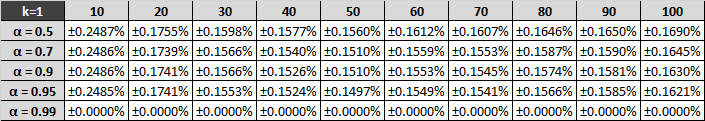
\includegraphics[width=\textwidth]{1_52_2}
\captionof{figure}{Error e IC 95\% en función de PCA para diversos $\alpha$ con $k=1$}
\end{center}
$ \\ $

\quad El resultado en forma de gráfica se presenta en la siguiente página.

\begin{center}
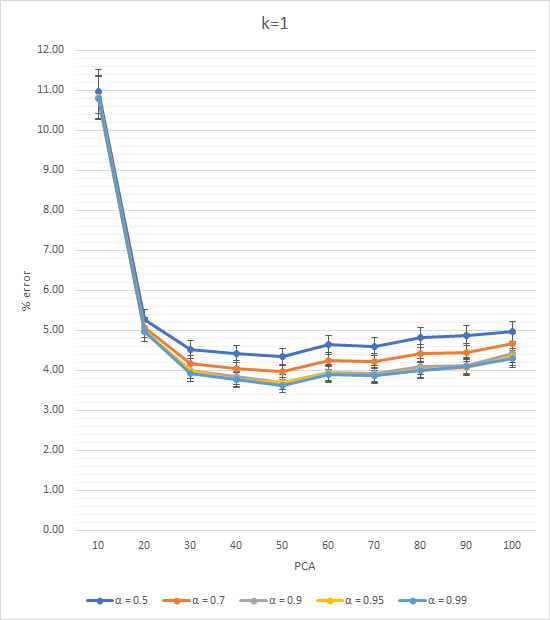
\includegraphics[width=\textwidth]{1_52_3}
\captionof{figure}{Gráfica del error en función de PCA para diversos $\alpha$ con $k=1$}
\end{center}
$ \\ $
\subsection{Ejericio 5.3}
\quad Los valores del suavizado son los mismos que en el ejercicio anterior.

\quad Las figuras de las siguientes páginas representan el resultado según las dimensiones reducidas de PCA en función del número de componentes.

\quad Se han vuelto a incluir los datos para $k=1$ con el fin de dar una visión más completa de los resultados. El mejor error es de un 2.20\%, obtenido para $k=9$ con 40 dimensiones de PCA y $\alpha = 0.9$ (marcado en amarillo).

\begin{center}
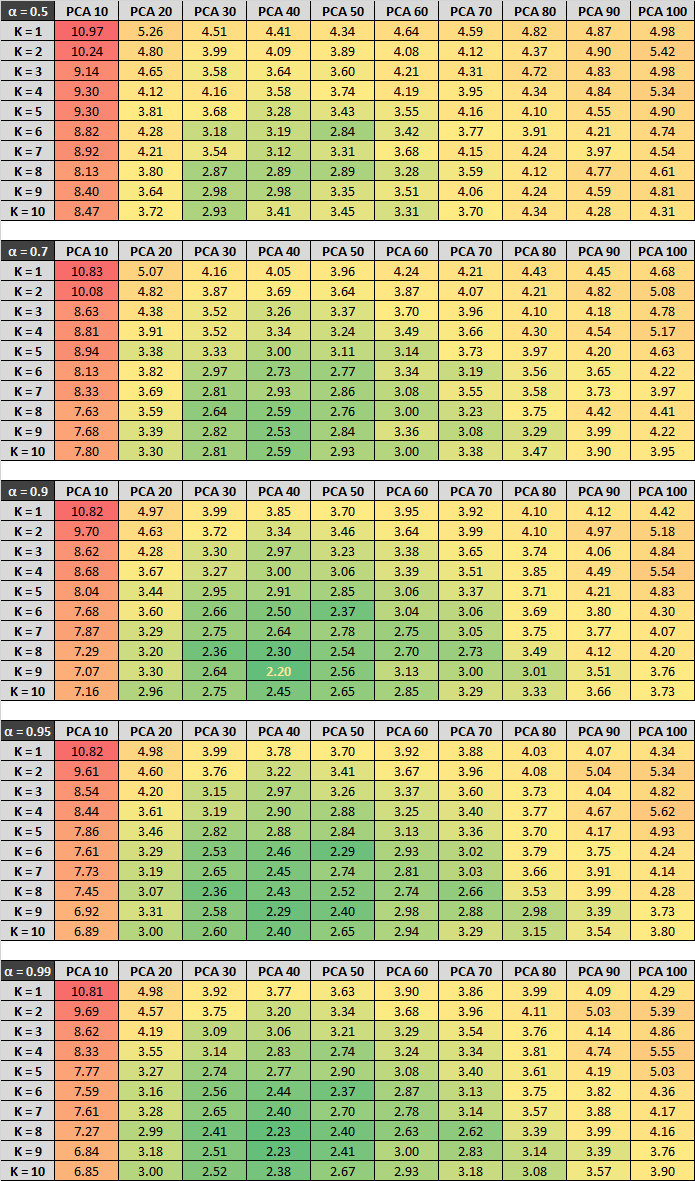
\includegraphics[width=330px]{1_tablas}
\captionof{figure}{Error según componentes y PCA para diversos suavizados en MNIST}
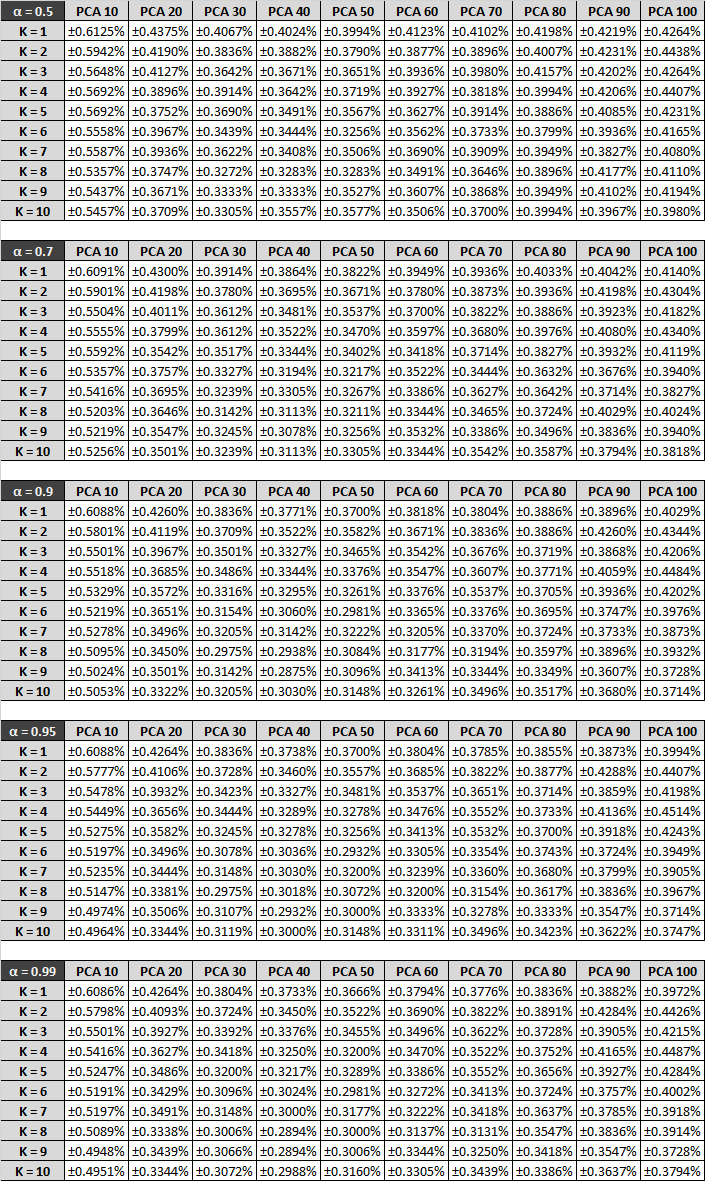
\includegraphics[width=330px]{1_ic}
\captionof{figure}{Intervalos de confianza al 95\% del error según componentes y PCA para diversos suavizados en MNIST}
\begin{landscape}
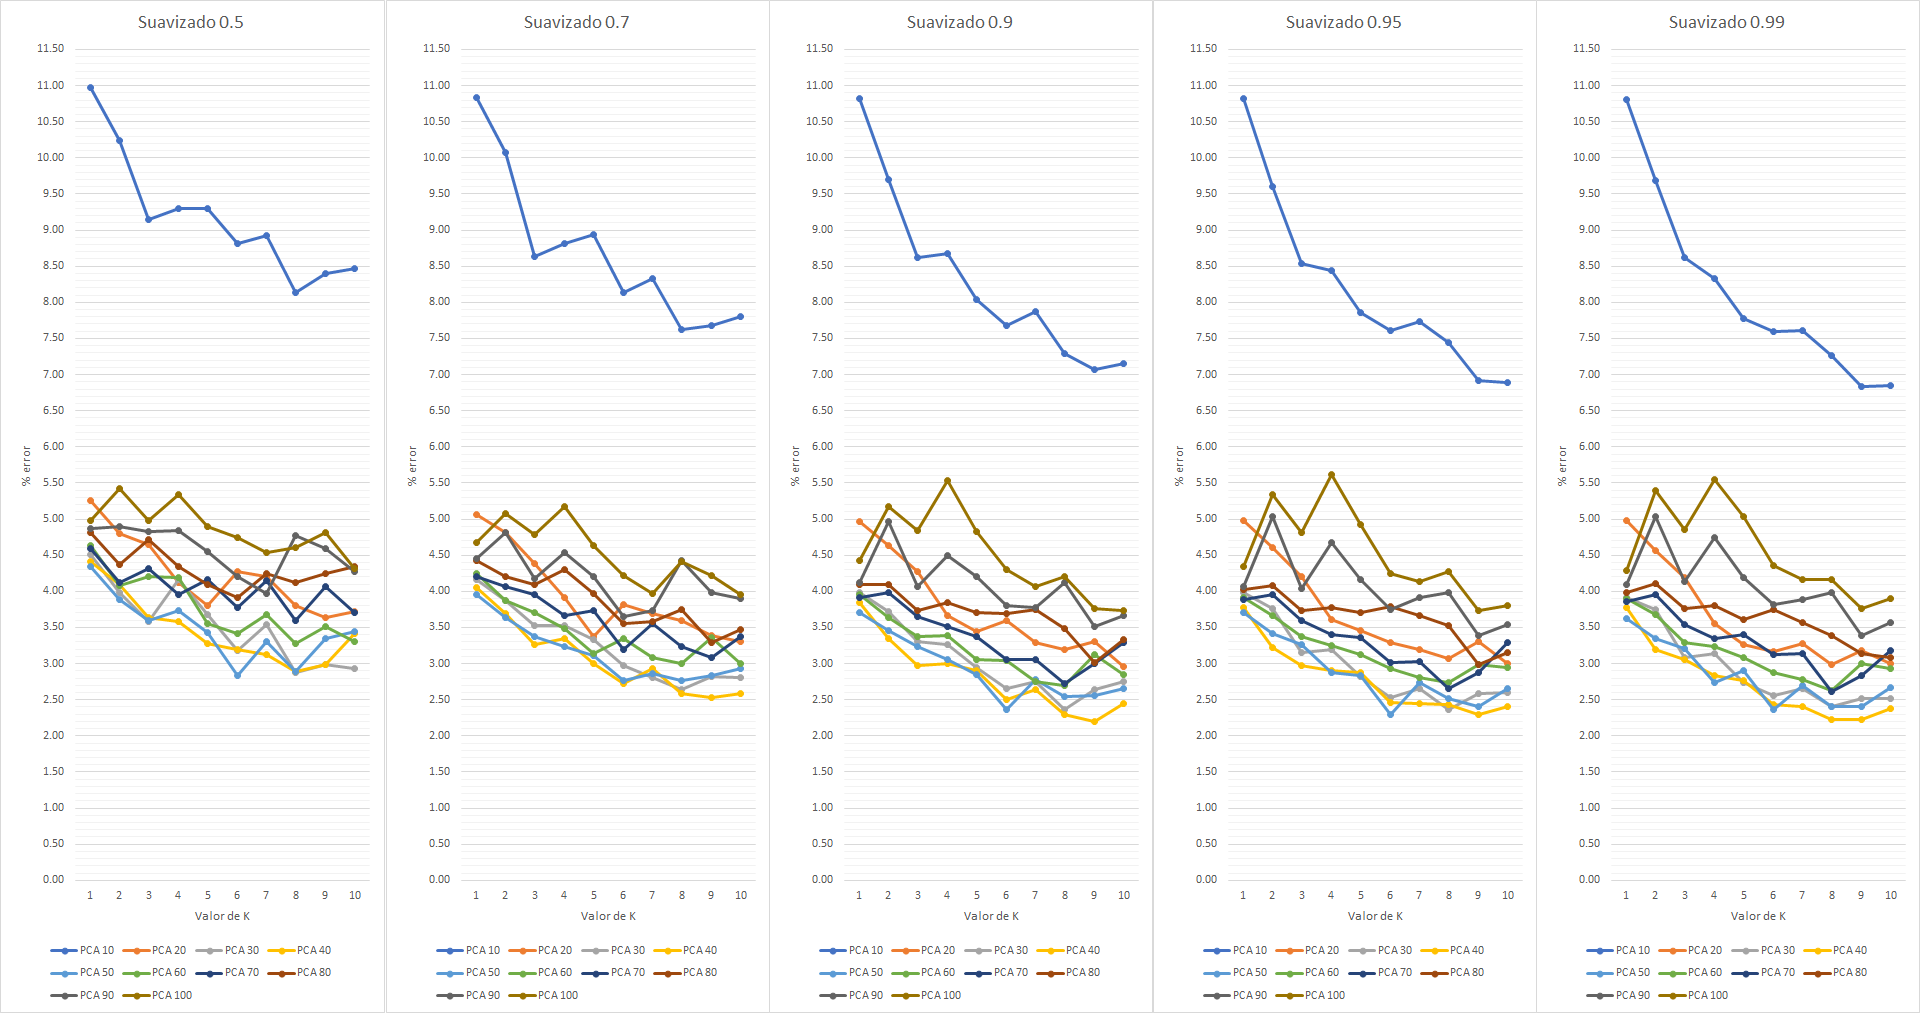
\includegraphics[height=300px]{1_graficas}
\captionof{figure}{Gráfica del error según componentes y PCA para diversos suavizados en MNIST}
\end{landscape}
\end{center}
$ \\ $

\section{Conclusiones}
\quad El valor del suavizado es importante a la hora de entrenar un modelo de mixtura de gaussianas. Un suavizado pequeño incrementa ligeramente la tasa de error con respecto a otros valores, mientras que un suavizado grande altera mucho el error tanto para entrenamiento como para test (véase $\alpha = 0.1$ en los resultados). De hecho, con un suavizado elevado, se puede comprobar en el entrenamiento cómo la mixtura de gaussianas "desaprende": debido al poco peso que tiene la matriz original con respecto a la matriz identidad, el error en cada ejecución aumenta. Esto a su vez se debe a que, si el valor de $\alpha$ es pequeño, se asume que los datos tienen poca covarianza ya que se le está dando más valor a la matriz identidad (únicamente varianza intraclase) que a la matriz calculada en la obtención de la matriz de covarianza (tanto varianza intraclase como varianza interclase), lo cual no tiene por qué ser cierto. Lo óptimo es que el valor del suavizado se encuentre entre 0.9 y 0.95, tal y como se ha podido comprobar en las tablas anteriores.

\quad En cuanto al error, el menor valor ha sido encontrado con la proyección a 40 dimensiones PCA, 9 componentes de la mixtura gaussiana y un valor del suavizado igual a 0.9. En general, pasadas unas dimensiones de proyección determinadas de PCA (entre 60 y 70 dimensiones), el error tiende a aumentar, así como si incrementamos en exceso las componentes de la mixtura. Los mejores errores se encuentran con entre 8 y 9 componentes de la mixtura gaussiana; con 10 componentes el error comienza a aumentar de nuevo. Esto no sigue del todo el esquema lógico a priori: 10 componentes deberían de ser el número ideal para clasificar 10 clases (en nuestro caso, 10 dígitos). Sin embargo, es posible que la representación de algunos números compartan ciertas características que permitan, por ejemplo, clasificar dos grupos de números mediante una componente de la mixtura, o clasificar tres grupos de números mediante dos componentes, lo que permitiría “ahorrarse” componentes de la mixtura gaussiana final.

\end{document}
